\documentclass{beamer}

\usepackage{amsmath, amssymb}
\usepackage{tikz-cd}
\usepackage{xcolor}
\usepackage{graphicx}

\title{MT222: Calculus II}
\author{\textbf{Miraj Samarakkody}}
\institute{Tougaloo College}
\date{03/31/2025}

\begin{document}

\begin{frame}
    \titlepage
\end{frame}




\begin{frame}{}
    \begin{center}
        \Huge{7.3 - Trigonometric Substitution}
    \end{center}
    
\end{frame}



\begin{frame}{Table of Trigonometric Substitiution}
    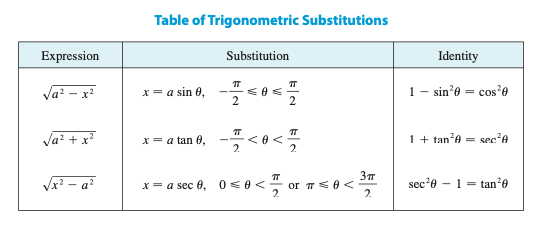
\includegraphics[scale=0.6]{figures/fig_1.png}
\end{frame}


\begin{frame}{Example 5}
    Evaluate \[\int \dfrac{dx}{\sqrt{x^2-a^2}},\] where \(a>0\). (Use Hyperbolic functions)
    
\end{frame}

\begin{frame}{Example 6}
    Find \[\int_{0}^{3\sqrt{3}/2}\dfrac{x^3}{(4x^2+9)^{3/2}}dx\]
\end{frame}

\begin{frame}{Example 7}
    Evaluate \[\int \dfrac{x}{\sqrt{3-2x-x^2}}dx\]
\end{frame}



\end{document}